\section{Administración del proyecto}

\subsection{Recursos humanos y materiales}

\begin{table}[ht]
\begin{center}
\begin{tabular}{|c|c|c|c|}
\hline
\textbf{Módulo} & \textbf{Material}                                                                     & \textbf{Cantidad} & \textbf{Costo (MXN)} \\ \hline
1.1             & Fuente de alimentación fija                                                           & 1                 & \$1500               \\ \hline
2.1             & CPU                                                                                   & 1                 & \$2000               \\ \hline
2.2 y 3.4       & \begin{tabular}[c]{@{}c@{}}Microcontrolador y componentes\\ electrónicos\end{tabular} & 2                 & \$600                \\ \hline
2.3             & Pantalla táctil                                                                       & 1                 & \$2000               \\ \hline
3.1             & Material para estructura                                                              & 1                 & \$1200               \\ \hline
3.2             & Guía lineal (1 riel y 2 bloques)                                                      & 2                 & \$1200               \\ \hline
3.5             & Servomotor y controlador                                                              & 1                 & \$6000               \\ \hline
3.6             & Sensor de fin de carrera                                                              & 3                 & \$200                \\ \hline
                &                                                                                       & Total             & \$15700              \\ \hline
\end{tabular}
\captionof{table}{Presupuesto estimado}
\label{tab:presupuesto}
\end{center}
\end{table}

\begin{center}
    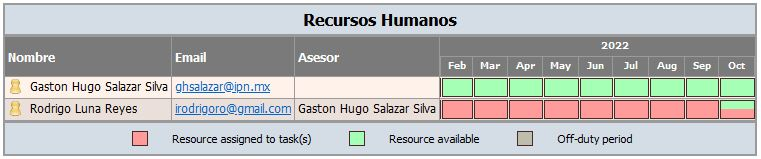
\includegraphics[scale=0.7]{imagenes/recursos_humanos_TT.JPG}
    \captionof{figure}{Recursos humanos disponibles para el proyecto}
    \label{fig:recursos_humanos}
\end{center}

\subsection{Planeación de actividades}
\begin{center}
    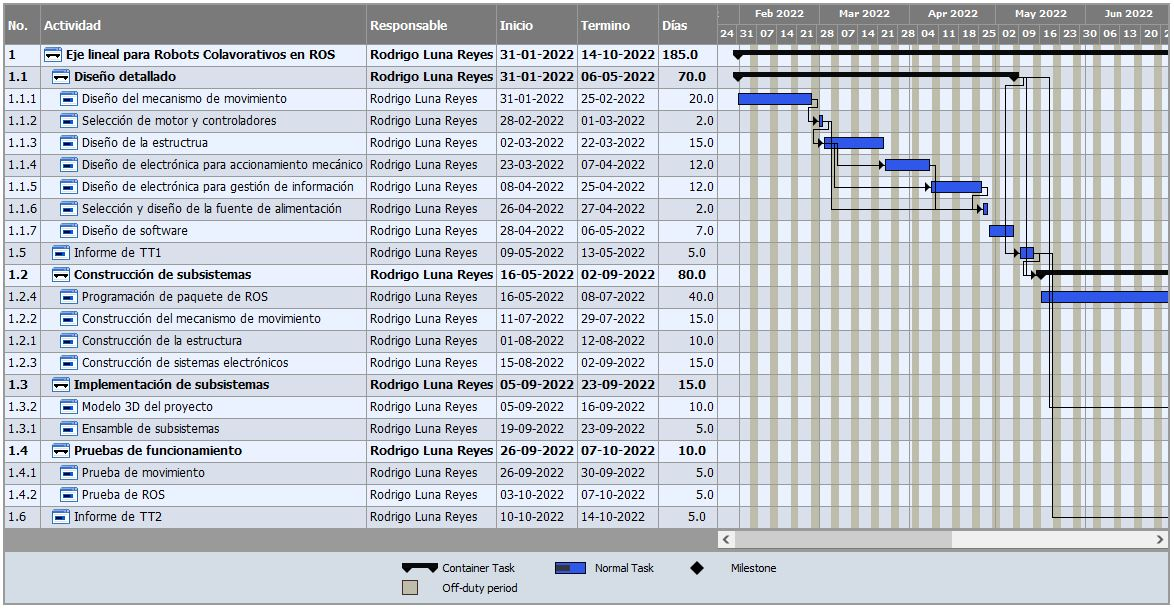
\includegraphics[scale=0.6]{imagenes/Cronograma TT1.JPG}
    \captionof{figure}{Cronograma para trabajo terminal 1}
    \label{fig:cronograma_tt1}
\end{center}
\begin{center}
    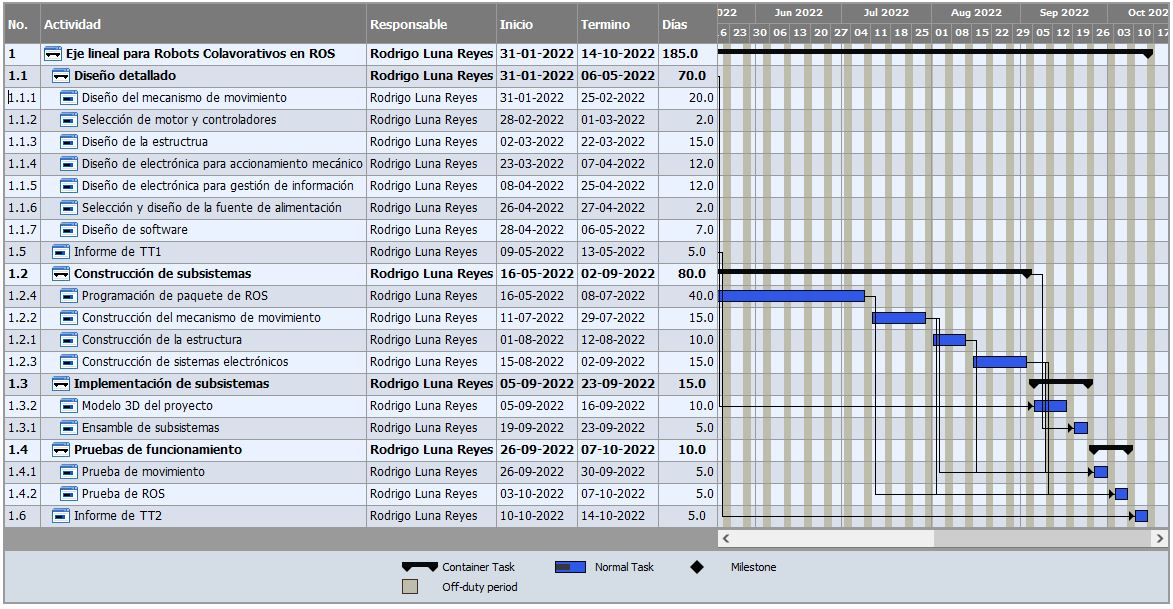
\includegraphics[scale=0.6]{imagenes/Cronograma TT2.JPG}
    \captionof{figure}{Cronograma para trabajo terminal 2}
    \label{fig:cronograma_tt2}
\end{center}